\documentclass{article}
\usepackage[german]{babel}
\usepackage{graphicx,hyperref,xcolor}

%%%%%%%%%% Start TeXmacs macros
\catcode`\>=\active \def>{
\fontencoding{T1}\selectfont\symbol{62}\fontencoding{\encodingdefault}}
\newcommand{\tminput}[2]{\trivlist{\item[\color{rgb:black,10;red,9;green,4;yellow,2}{#1}]{\color{blue!50!black}\mbox{}#2}}}
\newcommand{\tmoutput}[1]{#1}
\newcommand{\tmsession}[3]{{\tt#3}}
\newcommand{\tmstrong}[1]{\textbf{#1}}
\newcommand{\tmunfoldedio}[3]{\trivlist{\item[\color{rgb:black,10;red,9;green,4;yellow,2}{#1}]\mbox{}{\color{blue!50!black}#2}\item[]\mbox{}#3}}
%%%%%%%%%% End TeXmacs macros

\begin{document}

{\tmstrong{Vorlesung 6 24.05.2016}}

\

\href{/home/christian/Gedankenspeicher/Studium//Comp-NLD-1/Vorl6-A3-8.cpp}{Vorl6-A3-8.cpp}

\

\tmsession{shell}{default}{
  \tmoutput{Shell session inside TeXmacs pid = 13978}
  \tminput{Shell] }{g++ -o Vorl6-A3-8 Vorl6-A3-8.cpp \&\& ./Vorl6-A3-8 >
  V6-A3-8-E1.dat\\
  }
  \tminput{Shell] }{\ }
}

Plot gemitteltes R vs Epsilon

\tmsession{gnuplot}{default}{
  \tmoutput{This is a TeXmacs interface for GNUplot.}
  \tmunfoldedio{GNUplot] }{set yrange [0:1.5]; plot 'V6-A3-8-E1.dat' using 2:1
  with lines; \#beta0 = pi/4 , n =10, konz = 1, nsteps =
  5000}{\raisebox{0.0\height}{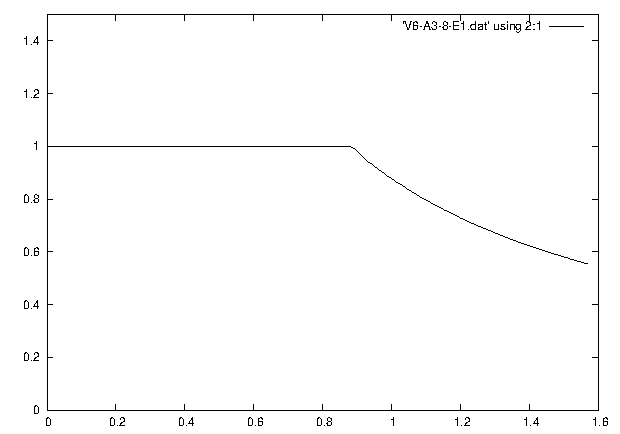
\includegraphics[width=10.411911321002231cm,height=7.288337924701561cm]{Vorlesung-6-1.pdf}}}
  \tminput{GNUplot] }{\ }
}

\

Animation mit Gnuplot aus C++ Programm heraus. Es wird sich ein Fenster
{\"o}ffnen, worin die Animation abgespielt wird. Zum Abbrechen der Animation
benutze Sitzung schlie{\ss}en

\tmsession{shell}{default}{
  \tmunfoldedio{Shell] }{g++ -o Vorl6-A3-9 Vorl6-A3-9.cpp \&\& ./Vorl6-A3-9
  \textbar  gnuplot}{{\scriptdead}}
  \tminput{Shell] }{\ }
}

\

\end{document}
